\documentclass[11pt]{article}
\usepackage{tikz}
\def\checkmark{\tikz\fill[scale=0.4](0,.35) -- (.25,0) -- (1,.7) -- (.25,.15) -- cycle;} 
\usepackage{proj} 	% pull in style header
\usepackage{array}
\usepackage{sectsty}

\lhead{ECE540: SoC Design with FPGA's}

%TODO: Put in coverpage from hw1, with tunnel vision image.  

%----------------------------------------------------------------------------------------
%	TITLE SECTION
%----------------------------------------------------------------------------------------


\newcommand{\horrule}[1]{\rule{\linewidth}{#1}} % Create horizontal rule command with 1 argument of height

\title{	
\normalfont \normalsize 
\textsc{\LARGE Portland State University}\\[1.5cm] % Name of your university/college
\textsc{\Large SoC Design With FPGAs}\\[0.5cm] % Major heading such as course name
\textsc{\large ECE540}\\[0.5cm] % Minor heading such as course title
%\textsc{Portland State University} \\ [25pt] % Your university, school and/or department name(s)
\horrule{1.2pt} \\[0.4cm] % Thin top horizontal rule
\huge Tunnel Vision \\ % The assignment title
\horrule{1.2pt} \\[0.5cm] % Thick bottom horizontal rule
}

%----------------------------------------------------------------------------------------
%	AUTHOR SECTION
%----------------------------------------------------------------------------------------
\begin{document}\raggedright
\author{Erik Rhodes \and Bhavana Dhulipala \and Rohan Deshpande \and Nikhil Patil} % Your name
\maketitle % Print the title
\thispagestyle{empty}
\cfoot{\textit{Page \thepage { of} \pageref{LastPage}}}
\lhead{ECE540: SoC Design}
\chead{github.com/rhodeser/tunnel-vision}
\rhead{Tunnel Vision}


\begin{figure}[h]\centering

\includegraphics[height=0.65\textwidth]{Images/start.png}
	%\caption{Gameplay Block Diagram}
		\label{start}
	\end{figure}



%
%\title{\textbf{ECE540: Final Project}\\Tunnel Vision}
%\author{Erik Rhodes and Bhavana Dhulipala}
%\date{February 4, 2014}

%\begin{document}
%	\maketitle{}
%	\thispagestyle{empty}
%	\newpage 
%	
%%		\thispagestyle{empty} % back of cover page is blank
%%		\vspace*{0.5\paperheight}
%%		\begin{center}
%%		{\it This page intentionally left blank}
%%		\end{center}
%%		\newpage
%		\begin{center}
%			\tableofcontents
%			\newpage
%	\end{center}


%Start of Document

% PUT IN CODE?
% put in design specs - Pictures: Top module, Hardware specifications?

\section{Introduction} 
Tunnel Vision is a racing game that can be played on the \textbf{Xilinx Nexys3 FPGA} board and be displayed on a VGA monitor.

\subsection{Gameplay}
The player tries to avoid hitting the walls as it travels down the tunnel by moving the vehicle left and right. The space in between the walls steadily decreases until the player hits a wall or obstacle. The score is based on the amount of time the vehicle remains ``alive'', and is displayed on the 7-segment display.

\subsection{Controls}
The player can move his vehicle by using the left and right pushbuttons on the Nexys3. When the game is over, hitting the middle button will reset the course. The top button starts the game and the bottom pushbutton pauses it. Different icons and speeds can be selected by toggling the switches on the board.

		\begin{figure}[h]\centering
		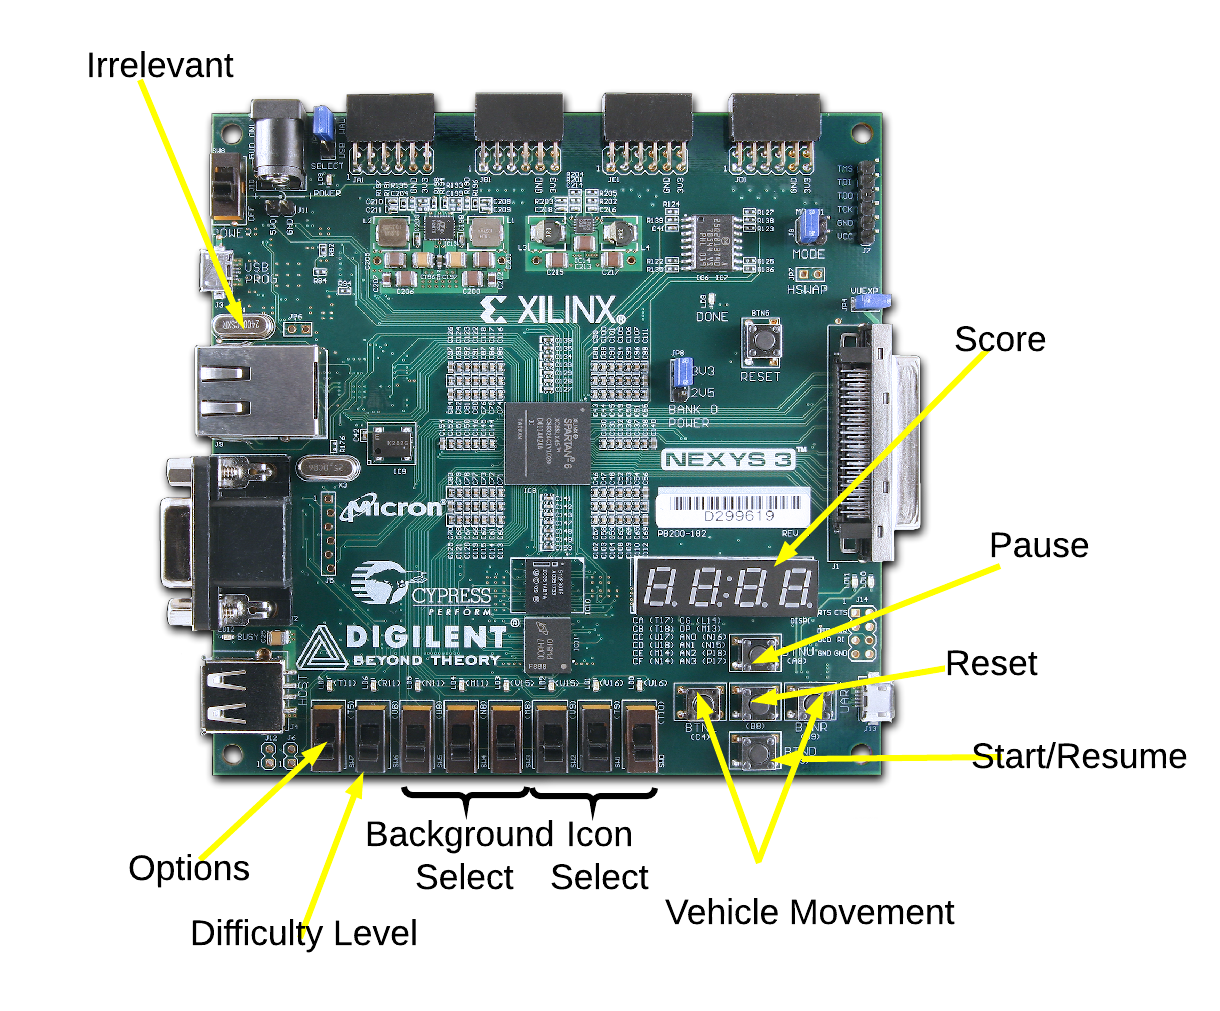
\includegraphics[height=0.8\textwidth, width=0.8\textheight]{Images/controls_mockup.png}
		\caption{Player Controls}
			\label{controls}
		\end{figure}	
	 	

\subsection{Features}
Tunnel Vision features both starting and ending screens. The courses are generated randomly through a pseudo-random number generator. Additionally, the LEDs are lit with certain patterns depending on the action the player is taking. If the player selects the harder difficulty, the score is incremented at a faster rate and with a multiplier, awarding them a higher score for the same distance traveled.
	


\section{Implementation}

	\begin{figure}[h]\centering
	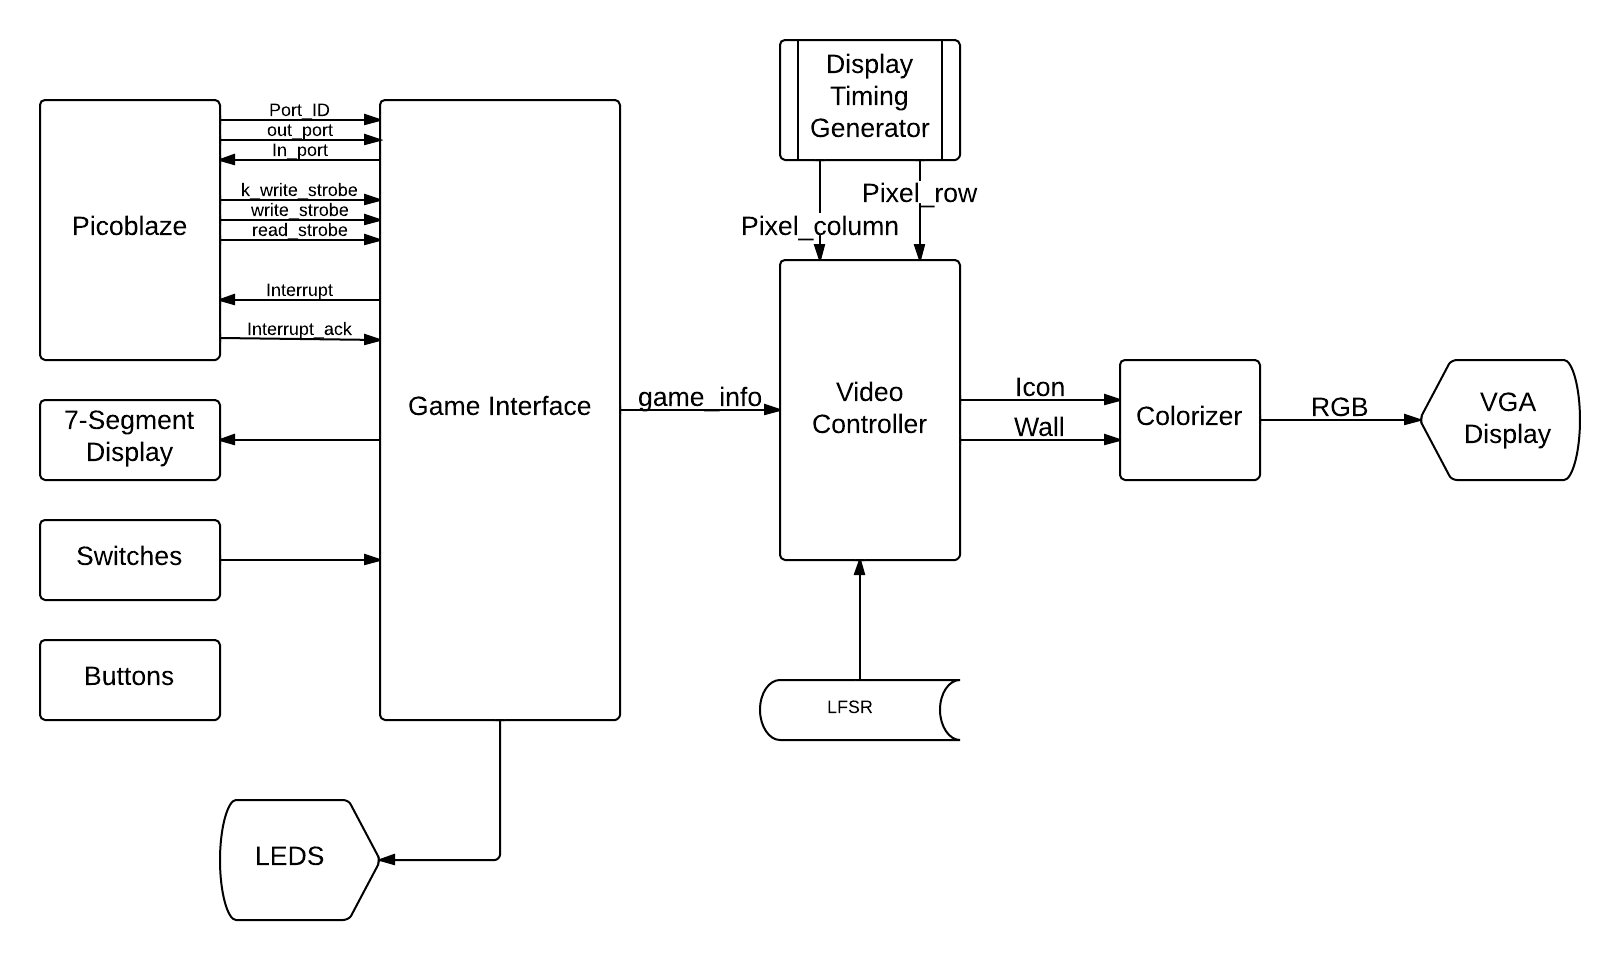
\includegraphics[height=0.7\textwidth, width=0.7\textheight]{Images/gameplay_diagram.png}
	\caption{Gameplay Block Diagram}
		\label{block_diagram}
	\end{figure}	
		
\subsection{Picoblaze}


		
		Picoblaze assembly code was used to implement the algorithm controlling the 
		vehicle's movement.
		Game logic, controls, score, levels, etc...
		




		
		%	\subsection{Forward}
			
Insert various code here

\begin{lstlisting}[caption=Sequence used manage orientation counter , label=loc_check]		
		LOAD	s0, 	LocX
		FETCH	s1,		SP_OLD_LOCX			;see if our current location is different
		COMPARE	s1,		s0						;if it is, we must be moving forward on a black line
		CALL	NZ,		clear_counter		;we can clear the orientation counter at this point 	
 \end{lstlisting}


	
\section{Video Controller Implementation}
	The video controller module was designed...
	The icon, wall, and different backgrounds implementation
	
%	\begin{figure}[t!]\centering
%	\includegraphics[height=0.5\textwidth]{video_controller.png}
%	\caption{Video Controller Overview}
%		\label{controller}
%	\end{figure}
		
		\subsection{Colorizer}
		

%		\begin{figure}
%		\centering
%		\begin{minipage}{.5\textwidth}
%			\centering
%		  	\includegraphics[width=.6\textwidth]{icon.png}
%		  		\caption{Icon Module}			
%			\label{icon}
%		\end{minipage}%
%		\begin{minipage}{.5\textwidth}
%		  	\centering
%			\includegraphics[width=.6\textwidth]{colorizer.png}
%			\caption{Colorizer Module}
%		  		\label{colorizer}
%		\end{minipage}
%		\end{figure}
%
%		\begin{figure}[t!]\centering
%		\includegraphics[height=0.3\textwidth]{colorizer_table.png}
%		\caption{Colorizer Table}
%			\label{colorizer_table}
%		\end{figure}
				

				
		\subsection{Icon}
		


%		\begin{figure}
%		\centering
%		\begin{minipage}{.5\textwidth}
%		  \centering
%		  \includegraphics[width=.6\textwidth]{icon_bitmap_3.png}
%		  \caption{Regular Image Translation}
%		  \label{reg_translation}
%		\end{minipage}%
%		\begin{minipage}{.5\textwidth}
%		  \centering
%		  \includegraphics[width=.6\textwidth]{icon_bitmap_4.png}
%		  \caption{Tilted Image Translation}
%		  \label{tilted_translation}
%		\end{minipage}
%		\end{figure}
					
		\begin{figure}[t!]\centering
		  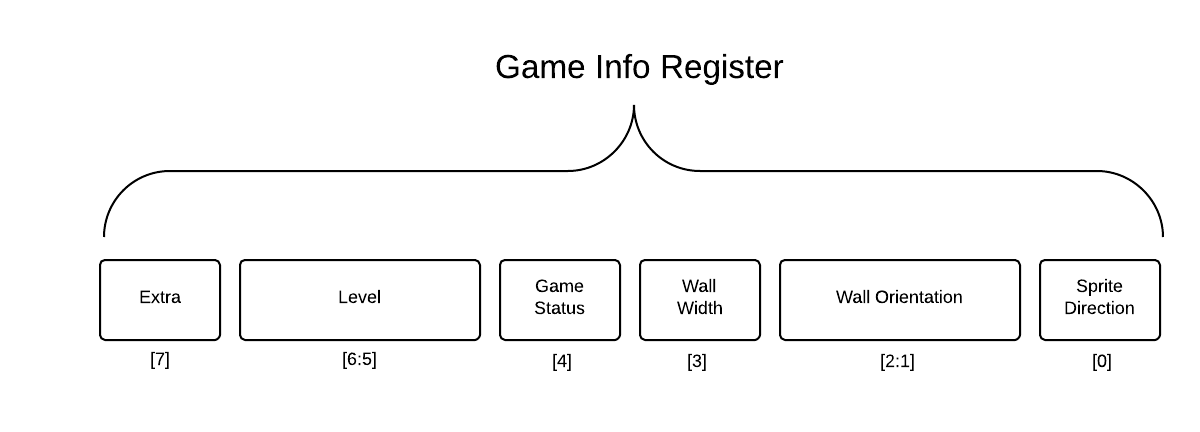
\includegraphics[width=.8\textwidth]{Images/game_info_bits.png}
		  \caption{Allocation of bits in game\_info register}
		  \label{game_info_bits}
		\end{figure}
		
		
		% first column
%\begin{minipage}[l]{0.5\textwidth}
%		\begin{itemize}

		
%\end{itemize}
%\end{minipage}\begin{minipage}[r]{0.5\textwidth}
%	\hspace{20pt}\includegraphics[width=0.9\textwidth]{../resources/mockup.png}
	
%	\hspace{50pt}Figure 1: Mockup of game screen


\section{Conclusion}
Length of time, github, results, etc.

	\subsection{Challenges}
		
		\begin{itemize}				
	
		\item Basically issues 
		
		\item problems we had
				
		\end{itemize}
	\subsection{Time Invested}

	
	
	%table "Division of Tasks" 
	\begin {table}[H]
	\begin {center} 

	\vspace{15pt}
	
	\begin{tabular}{||l|c|c||}\hline	
						& Erik Rhodes 	& Bhavana Dhulipala \\\hline
	bot\_ctrl.psm 		&	\checkmark 	&					\\\hline
	nexys\_bot\_if.v	&				&	\checkmark		\\\hline
	nexys3fpga.v		&	\checkmark	&	\checkmark		\\\hline	
	colorizer.v			&				&	\checkmark		\\\hline
	icon.v				&				&	\checkmark		\\\hline

	
	\end{tabular}
		\caption {Division of Tasks} \label{Division of Tasks}
	\end{center}
	\end{table}
	\subsection{Future Work}
	While our project completed all requirements and executed perfectly, there is still room for improvement. Future modifications would include:
	
	\begin{itemize}
	\item \textbf{Multiplayer Mode:} 
	\end{itemize}
\end{document}